% Q15：按固定候选 PDF 第 1 页重绘直三棱柱及 P 的位置；透视比例为示意。
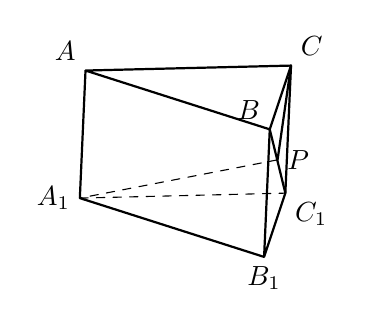
\begin{tikzpicture}[line cap=round,line join=round,scale=0.9]
  \coordinate (A) at (-1.75,1.55);
  \coordinate (B) at (0.85,0.72);
  \coordinate (C) at (1.15,1.62);
  \coordinate (A1) at (-1.83,-0.25);
  \coordinate (B1) at (0.77,-1.08);
  \coordinate (C1) at (1.07,-0.18);
  \coordinate (P) at (0.96,0.29);

  % 棱线；底部后侧棱 A1C1 按原图用虚线。
  \draw[thick] (A)--(B)--(C)--(A) (A)--(A1) (B)--(B1) (C)--(C1)
    (A1)--(B1)--(C1);
  \draw[dashed] (A1)--(C1);
  % BC1 上的动点 P，以及题目中的线段。
  \draw[thick] (B)--(C1) (C)--(P);
  \draw[dashed] (P)--(A1);

  \node[above left] at (A) {$A$};
  \node[above left] at (B) {$B$};
  \node[above right] at (C) {$C$};
  \node[left] at (A1) {$A_1$};
  \node[below] at (B1) {$B_1$};
  \node[below right] at (C1) {$C_1$};
  \node[right] at (P) {$P$};
\end{tikzpicture}
